\chapter{Lecture \thechapter{} of 01/04/2026}

\begin{proposition}[Book 1.4.6]

    Let $f : \R \to (-\infty,+\infty]$ closed proper convex, Consider $\Rc{f}$ and $\Lc{f}$ the recession cone and constancy space. Then 

    \begin{align*}
        \Rc{f} &= \set{d \in \Rn : \rf{f}(d) \le 0} \\
        \Lc{f} &= \set{d \in \Rn : \rf{f}(d) = 0}
    \end{align*}

\end{proposition}

\begin{proof}
    
    It follows from the definition of recession cone of a function that 

    \begin{align*}
        \Rc{f} &= \set{d \in \Rn : (d,0) \in \Rc{\epi{f}}} \\
            &= \set{d \in \Rn : (d,0) \in \epi{\rf{f}}} \\
            &= \set{d \in \Rn : \rf{f} \le 0}
    \end{align*}

    For the linearity space instead, we observe that $\Lc{f} = \Rc{f} \cap (-\Rc{f})$, $\rf{f}(d) \le 0$ and $\rf{f}(-d) \le 0$ for any $d \in \Lc{f}$. Then 

    \[ \rf{f}(0) = \rf{f}\left(\frac12 d + \frac12 (-d)\right) \le \frac12 \rf{f}(d) + \frac12 \rf{f}(-d). \]

    Observe that $\rf{f}(0) = 0$. Indeed, $\rf{f}(0) = \inf \set{w : (0,w) \in \Rc{\epi{f}}} = 0$ because we can take $w$ as negative as we want, but $f$ is proper, hence that infimum id 0. It follows that $\rf{f}(d) = \rf{f}(-d) = 0$ for any $d \in \Lc{f}$.

\end{proof}

\begin{proposition}[Book 1.4.7]
    
    Let $f : \Rn \to (-\infty,+\infty]$ be closed proper convex. Then, for every $x \in \dom{f}$, for any $d \in \Rn$ we have 

    \[ \rf{f}(d) = \sup_{\alpha > 0} \frac{f(x +\alpha d) - f(x)}{\alpha} = \lim_{\alpha \to +\infty} \frac{f(x + \alpha d) - f(x)}{\alpha}. \]

    Intuitively it gives a measure on ''how fast $f$ is diverging in the direction $d$''. 

\end{proposition}

\begin{proof}
    
    Not required.

\end{proof}

\section{Nonemptyness of instersection of closed sets}

Now we ask ourselfs a question: for $\set{C_k}_k$ a sequence of sets in $\Rn$ nested, i.e. $C_{k+1} \seq C_k$ for any $k$. We know that $C_k$ is compact for any $k$, then $\bigcap_k C_k \neq \emptyset$. Can we do similarly also if $C_k$ are only closed?

Why we ask such a question? 

\begin{example}
    
    Assume that we are looking for $\displaystyle\inf_{x \in X} f(x)$. Consider a sequence $\set{\gamma_k}_k \seq \Rn$, $\gamma_k \to \gamma^* = \inf_{x \in X} f(x)$. Does such a point exist? Define $X_k = \set{x : f(x) \le \gamma_k}$. One can show that if $\displaystyle\bigcap_k X_k$ is nonempty then there exists $x^*$ such that $f(x^*) = \gamma^*$.

\end{example}

\begin{example}
    
    Consider $A : \Rn \to \Rn$ a linear map, $C$ a closed set. Is the set $AC$ closed? Not always. Indeed, fix a sequence $\set{y_k}_k \seq AC$, $y_k \to \bar{y} \in \Rn$. Does $\bar{y} \in C$? Set $C_k = C \cap N_k$ where $N_k = \set{x : \norm{Ax - \bar{y}} \le \norm{y_k - \bar{y}}}$. One can show that if the intersection of $C_k$ is nonempty, then there exists a point $\bar{x} \in \bigcap_k C_k$ such that $A\bar{x} = \bar{y}$.

\end{example}

From now on, $C_k$ denotes a sequence of nested nonempty convex closed sets.

\begin{definition}
    
    We say that a sequence $\set{x_k}_k,\, x_k \neq 0$ is an \emph{asymptotic sequence} of $\set{C_k}_k$ if $\norm{x_k} \to +\infty$ and 

    \[ \frac{x_k}{\norm{x_k}} \to \frac{d}{\norm{d}} \]

    where $d \neq 0$, $d \in \bigcap_k \Rc{C_k}$. Intuitively, we can say that $\set{x_k}_k$ ''explodes only in a particular direction''.

\end{definition}

\begin{example}
    
    Consider $C_k = \set{x : x \ge k}$, then $d = 1 \in \bigcap_k \Rc{C_k}$. Moreover, any unbounded sequence in $\R$ is asymptotic, as $\R$ has a unique direction in which a sequence can escape.

\end{example}

\begin{remark}
    
    Given any unbounded sequence $\set{x_n}_n \seq \R^d$, there exists a subsequence $\set{x_{n_k}}_k$ that is asymptotic, because every cluster point of $\set{x_n/\norm{x_n}}_n$ is a common recession direction for each $C_k$.

\end{remark}

\begin{definition}[Retractive asymptotic sequence]

    An asymptotic sequence $\set{x_k}_k$ of $\set{C_k}_k$, with $d$ as asymptotic direction is \emph{retractive} if there exists a $\bar{k}$ big enough such that $x_k - d \in C_k$ for any $k > bar{k}$.

\end{definition}

\begin{definition}
    
    A sequence $\set{C_k}_k$ is \emph{retractive} if all its asymptotic sequence are retractive. A set $C \seq \Rn$ is retractive in the same way.

\end{definition}

\begin{example}
    
    The sequence $C_k = \set{x : x \ge k}$ is not retractive because there exist a sequence $\set{x_k}_k$ such that $x_k - d \notin C_k$, e.g. $x_k = k, d = 1$, so $x_k - d = k - 1 \notin C_k$.

    Let $C_k = \set{(x,y) \in \R^2 : \abs{x} \le \frac1k}$. Then 

    \[ \bigcap_k C_k = \set{(0,y): y \in \R} \neq \emptyset. \]

    This sequence is retractive, as the only direction of escape is $y$. 

    \begin{figure}[ht!]
        \centering
        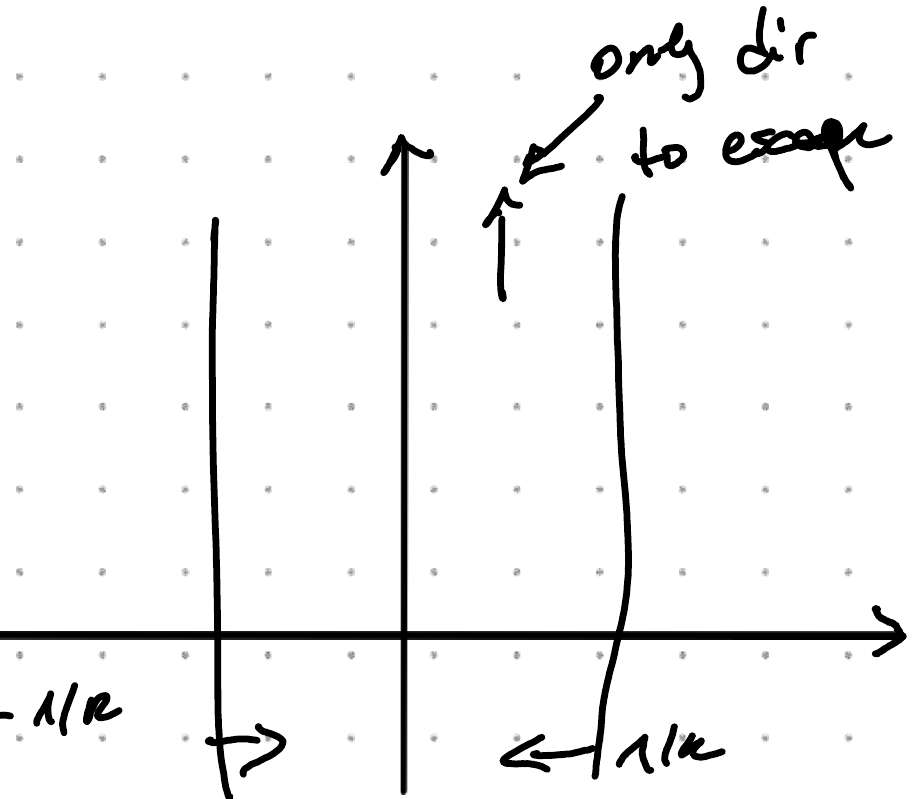
\includegraphics[width=0.8\textwidth]{img/retractive.png}
        \caption{Visual intuition for the example}
    \end{figure}

\end{example}

\begin{remark}
    
    Assume $\set{C_k^1}_k$, $\set{C_k^2}_k$, \dots, $\set{C_k^m}_k$ to be $m$ families of nested closed convex nonempty sets. Then define

    \begin{align*}
        N_k &= C_k^1 \cap \dots \cap C_k^m \\
        T_k &= C_k^1 \times \dots \times C_k^m.
    \end{align*}

    If each sequence is retractive and $N_k \neq \emptyset$ then $\set{N_k}_k$ and $\set{T_k}_k$ are retractive.

\end{remark}

\begin{proposition}
    Polyhedral sets are retractive.
\end{proposition}

\begin{proof}
    Corollary of the above remark.
\end{proof}

\begin{proposition}
    A retractive nested sequence of nonempty closed convex sets has nonempty interior.
\end{proposition}

\begin{proof}
    Scketched in class, not reported here.
\end{proof}

\begin{example}
    
    Retractiveness is \emph{not} a necessary condition: consider the sequence

    \[ C_k = \set{(x,y) \in \R^2 : y \ge x^2 - \frac1k}. \]

    Then the intersection is nonempty but $C_k$ is not retractive: the only direction of escape is $(0,1)$, but if we take a point on the boundary of each $C_k$ we go out of the set.

\end{example}

The question now is: how can we easly prove retractiveness? The answer is in the following:

\begin{proposition}[Book 1.4.11]
    
    Denote $R = \bigcap_k \Rc{C_k}$ and $L = \bigcap \Lc{C_k}$. Then 

    \begin{enumerate}
        \item[a)] Il $R = L$ then $\set{C_k}_k$ is retractive. Furthermore it holds true that 
            \[ \bigcap_k C_k = L + \tilde{C} \]
            where $\tilde{C}$ is a nonempty compact set;
        \item[b)] Fix $X \seq \Rn$ retractive, closed and convex. Assume that the sets $\overline{C}_k = X \cap C_k$ are nonempty and $\Rc{X} \cap R \subset L$. Then $\overline{C}_k$ is retractive.
    \end{enumerate}

\end{proposition}

\begin{proof}
    Not required.
\end{proof}

\begin{proposition}[Existance of solution of convex quadratic problems, book 1.4.12]

    Let $Q \in \R^{n \times n}$ be SPD, $c \in \Rn$, $a_1,\dots, a_m \in \Rn$, $b_1,\dots,b_m \in \R$. Let $f : \Rn \to \R$, $x \mapsto x^\top Q x + c^\top x$, and $X = \set{x \in \Rn : a_j^\top x \le b_j,\, \forall \, 1 \le j \le m}$. Assume $\inf_{x \in X} f(x)$ to be finite. Then there exists $x^* \in X$ such that 

    \[ f(x^*) = \inf_{x \in X} f(x). \]
    
\end{proposition}

\begin{proof}
    
    Let $f^* = \inf_{x \in X} f(x)$. Let $\set{\gamma_k}_k \seq \R$ such that $\gamma_k \to f^*$ as $k \to +\infty$. Define $\overline{C}_k = X \cap \set{x : f(x) \le \gamma_k}$. Let $\Rc{X}$ be the recession cone of $X$, $R = \Rc{\bigcap_k C_k}$, $L = \Lc{\bigcap_k C_k} (= \Rc{C_k} = \Lc{C_k})$ since we already know that the sublevel sets share all the same recession cone. In a previous example we computed 

    \begin{align*}
        R &= \set{d : Qd = 0,\, c^\top d \le 0} \\
        L &= \set{d : Qd = 0,\, c^\top d = 0} \\
        \Rc{X}  &= \set{d : a_j^\top d \le 0,\, \forall\, 1\le j\le m}.
    \end{align*}

    Take $d \in \Rc{X} \cap R$, assume $d \notin L$. Then $Qd = 0$, $c^\top d < 0$, $a_j^\top d \le 0$ for all $j$, but then $f(x + \alpha d) \to -\infty$ as $\alpha \to +\infty$, which contraddicts the fact that $f^*$ is finite. Hence $\Rc{X} \cap R \seq L$, so by the previous theorem, $\set{\overline{C}_k}_k$ is retractive, and so there exists $x^* \in \bigcap_k \overline{C}_k$ such that $f(x^*) = f^*$.

\end{proof}

